\chapter{Calendar Interface}
\section{Einleitung}
Im folgenden Diagramm ist die Architektur und Integration des Calendar Interface in die Stundenplan App dargestellt.
\begin{figure}[htb]
    \centering
    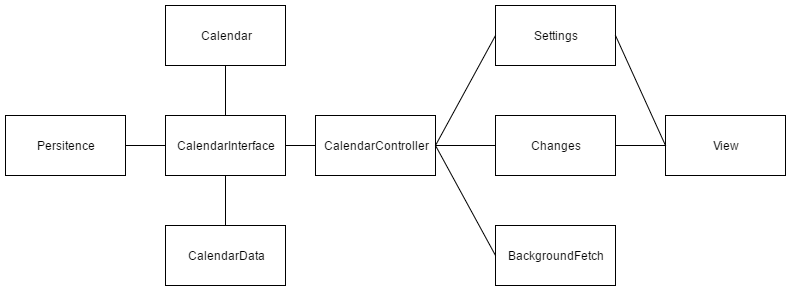
\includegraphics[width=\textwidth]{CalendarInterface_Diagram}
    \caption{CalendarInterface Diagramm}
\end{figure}

Das Calendar Interface besteht aus folgenden drei Klassen:
\begin{itemize}
     \item CalendarController
     \item CalendarInterface
     \item CalendarData
\end{itemize}

Im Folgenden wird auf die Klassen genauer eingegangen.

\newpage
\section{CalendarController}
Der CalendarController ist der Controller für das Calendar Interface. Über ihm wird auf das Interface zugegriffen.

Im Folgenden wird auf die wichtigsten Methoden eingegangen:
\begin{itemize}
     \item createCalendar()
     \item removeCalendar()
     \item createAllEvents()
     \item updateAllEvents()
     \item removeAllEvents()
     \item CalendarRoutine()     
\end{itemize}

Jede Methode überprüft ob die Berechtigung gewährt wurde und reagiert entsprechend.

\subsection{createCalendar}
Erzeugt den Kalender falls die Berechtigung vorhanden ist. Falls er erzeugt wurde werden die Events mit createAllEvents in den Kalender geschrieben. Als Rückgabewert gibt er den Berechtigungsstatus zurück. Es gibt drei Rückgabewerte:
\begin{itemize}
     \item authorized \\[0.5em]
     Bedeutet das der Nutzer die Berechtigung erteilt hat und der Kalender angelegt wurde oder bereits angelegt war.
     \item notDetermined \\[0.5em]
     Bedeutet das die Berechtigung gerade abgefragt wird.
     \item denied \\[0.5em]
     Bedeutet das die Berechtigung verweigert wurden.
\end{itemize}

\subsection{removeCalendar}
Löscht den Kalender mit Hilfe des CalendarInterface.

\subsection{createAllEvents}
Erzeugt die aus den Vorlesungen die Events, die anschließend mit Hilfe des CalendarInterface in den Kalender geschrieben werden.
Falls der Kalender noch nicht erzeugt wurde wird er angelegt.
Die EventID's werden persistent gespeichert.

\subsection{updateAllEvents}
Ermittelt welche Art von Änderung vorliegt und passt die Events mit Hilfe des CalendarInterface entsprechend an.
Die EventID's werden persistent gespeichert.

\subsection{removeAllEvents}
Holt sich für die übergebenden Vorlesungen die EventID's und löscht die entsprechenden Events mit Hilfe des CalendarInterface.
Die Änderungen an den EventID's werden persistent gespeichert.

\subsection{CalendarRoutine}
Aktualisiert die Vorlesungen im Kalender. Dazu holt sie sich die abgewählten und neu ausgewählten Vorlesungen und übergibt sie der removeAllEvents oder createAllEvents-Methode.

\newpage
\section{CalendarInterface}
Dies ist die Klasse die direkt auf den Kalender zugreift. 

Im Folgenden wird auf die wichtigsten Methoden eingegangen:
\begin{itemize}
     \item createCalenderIfNeeded()
     \item removeCalendar()
     \item createEvent()
     \item updateEvent()
     \item removeEvent()
     \item saveIDs()
\end{itemize}

\subsection{createCalenderIfNeeded}
Erzeugt den Kalender falls er nicht bereits vorhanden ist. Gibt einen Boolean-Wert zurück ob der Kalender angelegt wurde.

\subsection{removeCalendar}
Löscht den Kalender falls dieser vorhanden ist. Gibt einen Boolean-Wert zurück ob das Löschen erfolgreich war.

\subsection{createEvent}
Schreibt das übergebende Event in den Kalender.

\subsection{updateEvent}
Das zu der EventID dazugehörige Event wird mit den entsprechend Werten des übergebenen Event angepasst.

\subsection{removeEvent}
Löscht das übergebene Event. Gibt einen Boolean-Wert zurück ob das Löschen erfolgreich war.

\subsection{saveIDs}
Speichert die EventIDs der Vorlesungen und Änderungen.

\newpage
\section{CalendarData}
Die CaledenarData-Klasse dient dazu, die EventIDs der Vorlesungen und Änderungen getrennt in Dictonarys zu speichern.
Die Dictonarys bestehen aus einer Zuordnung von einer ID einer Vorlesung zu mehreren EventIDs.

